
\section{\esp Introdução}

Dentro de grafos simples existem diversos conceitos e aplicações que vêm sido estudadas ao longo de décadas. Dentro dos conceitos mais clássico, temos a definição de caminho, que resumidamente é uma sequência de vértices onde arestas não são repetidas. 

Um comportamento interessante de caminhos são os caminhos disjuntos, que são dois ou mais caminhos de um mesmo grafo, que não possuem nenhuma aresta em comum entre si. Uma vez entendido esse conceito, torna-se interessante encontrar o número máximo de caminhos disjunto de um grafo.

Para tentar solucionar esse problema, foi proposto pensar em um grafo ponderado, onde todas arestas possuem peso igual. Tendo esse novo grafo, ao calcular o fluxo máximo aparenta ser possível encontrar esse número máximo. As seções seguintes descrevem a implementação, os testes e conclusões sobre resultados encontrados.

\section{\esp Implementação}

Para desenvolver a solução do trabalho, utilizamos a linguagem Java. Ela foi escolhida por ser uma linguagem que permite implementar facilmente orientação de objetos e ser relativamente rápida. 

Foram criadas diferentes classes que se complementam na solução, das quais se destacam a classe \textit{Grafo}, que modela um grafo qualquer e possui os métodos necessários para resolver o problema e as classes utilitárias \textit{Edge} e \textit{Tuple}, usadas para encapsular os conceitos de vértice e tuplas, facilitando a implementação. Todas as classes foram escritas de forma a rodar em uma única \textit{Thread} de execução.

\subsection{\esp Classe Grafos}

A classe Grafo foi desenvolvida para ser a principal estrutura de dados utilizada durante o trabalho. Apesar dos exercícios serem para grafos direcionados, implementamos a classe de forma que ela também para grafos não direcionados, o atributo \textit{isDirectional} faz o controle dessa característica do grafo, tendo o \textit{default} como verdadeiro.

Utilizamos de uma matriz de adjacência para armazenar as arestas e seus respectivos pesos, dentro da classe a matriz pode ser acessada por meio do atributo \textit{edgesWeights}. Fora a facilidade de utilização e implementação, a matriz de adjacência permite extrair todas as arestas que saem de um dado vértice, por meio do método \textit{getAllEdgesFromNode}. dada uma origem é possível atingir outro vértice, por meio da busca em largura.

Para os construtores da classe, definimos uma estrutura de arquivo que pode ser importada pelo construtor para facilitar os testes, neste arquivo, temos o cabeçalho, com uma linha e três valores que ditam quantos vértices o grafo possui e de qual à qual vértice os caminhos serão procurados. No corpo, cada linha representa uma aresta direcional, com dois valores representando quais vértices a aresta liga, sendo o primeiro a origem e o segundo o destino.

Fora os métodos explicitados acima, construímos outros métodos auxiliares que utilizam pesos na matriz de adjacência, adicionar vértices ou arestas, e outras funções que julgamos necessárias.

\subsection{\esp Algoritmo} \label{sec:algoritmo}

Para buscar os caminhos disjuntos em um grafo, interpretamos o grafo direcional como um problema de fluxo máximo e implementamos uma variação do algoritmo de Edmonds-Karp, mas como todas as arestas possuem a mesma capacidade, utilizar as arestas de retorno de uma rede residual não geraria nenhum aumento no fluxo máximo, buscar os caminhos mais curtos por meio de uma busca em largura é suficiente para obter o resultado ótimo.

Como já comentado acima, nossa implementação é uma variação do método desenvolvido por Edmonds-Karp para obter o fluxo máximo de uma rede de fluxo. É gerada uma cópia do grafo original e buscamos o menor caminho em quantidade de arestas, por meio de uma busca em largura, enquanto existirem caminhos e os adicionamos na resposta. Cada aresta pode ser usada uma única vez por conta da capacidade constante da rede de fluxo, então após utilizadas, todas as arestas de um caminho são removidas da cópia.

\section{\esp Experimentos} \label{sec:experimentos}

Para realizar os experimentos foram desenvolvidos alguns grafos para testes, baseados em exemplos mostrados em sala de aula, para este relatório vamos focar nos representados nas figuras \ref{fig:K5} e \ref{fig:G}. Nas figuras, a origem foi sempre o vértice \textit{s} e o destino o vértice \textit{t} arestas que foram utilizadas para algum caminho foram representadas em vermelho.

No grafo \textit{K5}, foram encontrados 4 caminhos, um direto de \textit{s} a \textit{t} e os outros três passando por um dos outros vértices do grafo. É interessante notar que apesar de ser possível realizar loops, como o passeio \textit{s 1 2 1 t} ao invés do \textit{s 1 t} por conta do uso da busca em largura, eles são evitados.

No grafo \textit{G}, foram encontrados 3 caminhos, que novamente por conta da busca pelos menores caminhos evitou casos onde 2 ou menos caminhos seriam encontrados.

\begin{figure}
\centering
\begin{minipage}{.3\textwidth}
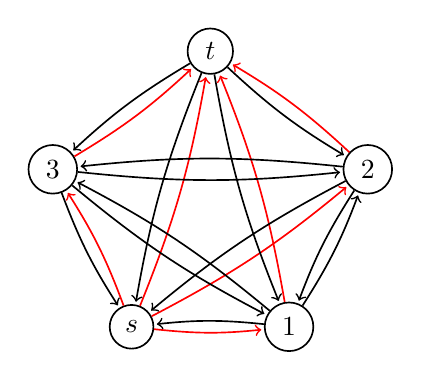
\begin{tikzpicture}[->,shorten >=1pt,auto,node distance=4.5cm,
                    semithick]
\def \margin {20}
\node[draw, circle] (1) at (1,0) {$s$};
\node[draw, circle] (2) at (3,0) {$1$};
\node[draw, circle] (3) at (4,2) {$2$};
\node[draw, circle] (4) at (0,2) {$3$};
\node[draw, circle] (5) at (2,3.5) {$t$};

\draw[->,red] (1) to [bend right=6] (2);
\draw[->,red] (1) to [bend right=6] (3); 
\draw[->,red] (1) to [bend right=6] (4); 
\draw[->,red] (1) to [bend right=6] (5); 
\draw[->] (2) to [bend right=6] (1); 
\draw[->] (2) to [bend right=6] (3); 
\draw[->] (2) to [bend right=6] (4); 
\draw[->,red] (2) to [bend right=6] (5); 
\draw[->] (3) to [bend right=6] (1);
\draw[->] (3) to [bend right=6] (2);
\draw[->] (3) to [bend right=6] (4);
\draw[->,red] (3) to [bend right=6] (5);
\draw[->] (4) to [bend right=6] (1);
\draw[->] (4) to [bend right=6] (2);
\draw[->] (4) to [bend right=6] (3);
\draw[->,red] (4) to [bend right=6] (5);
\draw[->] (5) to [bend right=6] (1);
\draw[->] (5) to [bend right=6] (2);
\draw[->] (5) to [bend right=6] (3);
\draw[->] (5) to [bend right=6] (4);

\end{tikzpicture}
\caption{K5} \label{fig:K5}
\end{minipage}%
\begin{minipage}{.5\textwidth}
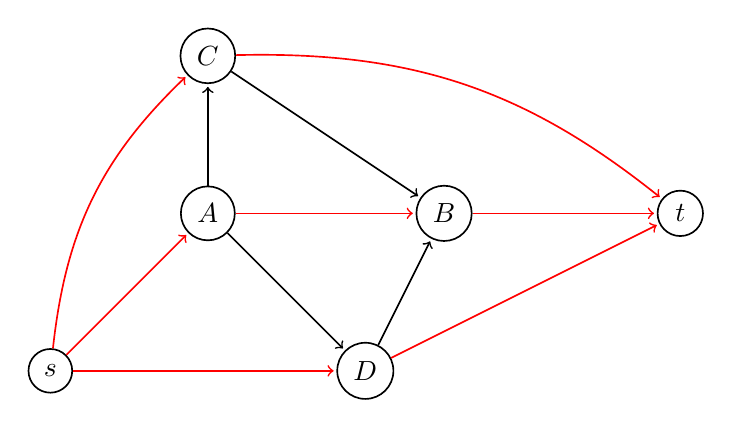
\begin{tikzpicture}[->,shorten >=1pt,auto,node distance=4.5cm,
                    semithick]
\def \margin {20}
\node[draw, circle] (A) at (0,0) {$s$};
\node[draw, circle] (B) at (2,2) {$A$};
\node[draw, circle] (C) at (5,2) {$B$};
\node[draw, circle] (D) at (2,4) {$C$};
\node[draw, circle] (E) at (4,0) {$D$};
\node[draw, circle] (F) at (8,2) {$t$};

\draw[->,red] (A) to  (B);
\draw[->,red] (A) to [bend left=20] (D); 
\draw[->,red] (A) to (E); 
\draw[->,red] (B) to (C); 
\draw[->] (B) to (D); 
\draw[->] (B) to (E); 
\draw[->,red] (C) to (F); 
\draw[->] (D) to (C); 
\draw[->,red] (D) to [bend left=20] (F); 
\draw[->] (E) to (C); 
\draw[->,red] (E) to (F);

\end{tikzpicture}
\caption{G} \label{fig:G}
\end{minipage}
\end{figure}

\section{\esp Conclusão}

Caminhos disjuntos possuem diversas aplicações e encontrá-los em um grafo grande pode se apresentar como um problema, portanto um algoritmo que consiga calcular esses caminhos de maneira ótima computacionalmente pode ser usado em diversas aplicações, desde redes de computadores até logística de entrega.

Utilizando conceitos que foram usados em outros problemas conseguimos transformar o problema e adaptar soluções já existentes para um novo problema de forma a facilitar a resolução garantindo a eficiência do método.
